\documentclass[aspectratio=169]{beamer}
\usepackage{listings}
\usepackage{listings}
\usepackage{xcolor}
\newlength{\edgelen}
\setlength{\edgelen}{0.3cm}
\newcommand\blank[1]{\rule[-.2ex]{#1}{.4pt}}
\usepackage{tikz}
\usetikzlibrary{shapes,arrows,positioning}
\usepackage[dvipsnames]{xcolor}

\usetikzlibrary{shapes.callouts, positioning, arrows.meta,calc,backgrounds}

% Use plain theme with no decorations
\usetheme{default}
\setbeamertemplate{navigation symbols}{}
\setbeamertemplate{footline}{}
\setbeamertemplate{headline}{}

% Define Java code style
\lstdefinestyle{pythonstyle}{
    language=Python,
    basicstyle=\ttfamily\small,
    keywordstyle=\color{blue}\bfseries,
    commentstyle=\color{gray}\itshape,
    stringstyle=\color{red},
    numberstyle=\tiny\color{gray},
    numbers=left,
    stepnumber=1,
    numbersep=8pt,
    backgroundcolor=\color{white},
    showspaces=false,
    showstringspaces=false,
    showtabs=false,
    frame=single,
    tabsize=4,
    captionpos=b,
    breaklines=true,
    breakatwhitespace=false
}


\title{Tri fusion (Merge-sort) - Récursion illustrée}
\subtitle{Étapes de la récursion}
\author{Algorithmes et Pensée Computationnelle \newline \newline  {\small UNIL — École des Sciences Criminelles}}
\date{}

\begin{document}

\begin{frame}
\titlepage
\end{frame}

\begin{frame}[fragile]{Code}
\begin{center}
\begin{lstlisting}[style=pythonstyle, caption={Merge sort — Python}]
def sort(arr):
    if len(arr) <= 1:
        return arr
    
    mid = len(arr) // 2
    left = sort(arr[:mid])
    right = sort(arr[mid:])
    
    return merge(left, right)
\end{lstlisting}
\end{center}

La fonction \texttt{merge} prend deux listes triées comme paramètres et renvoie une liste triée qui est la fusion de ces deux listes. La fonction \texttt{merge} a donc une complexité de $O(n)$.
\end{frame}



\begin{frame}[fragile]{Étape 1}

\resizebox{0.892\textwidth}{!}{%

\begin{tikzpicture}[
    node distance=1cm,
    box/.style={rectangle, draw=black, thick, minimum width=3cm, minimum height=1cm, align=center}
]

\draw[draw = white] (-7,-6) rectangle (7,6);  % invisible bounding box

% Top node
\node[box] (root) at (1,5) {
  \texttt{\shortstack[l]{sort([8,4,7,10,6,1,2,5]) \\ \textcolor{blue}{return:}}}
};

\end{tikzpicture}
}
\end{frame}











\begin{frame}[fragile]{Étape 2}

\resizebox{0.892\textwidth}{!}{%
\begin{tikzpicture}[
    node distance=1cm,
    box/.style={rectangle, draw=black, thick,
                minimum width=1cm, minimum height=1cm, align=center}
]

\draw[draw = white] (-7,-6) rectangle (7,6);  % invisible bounding box

% Top node
\node[box] (root) at (1,5) {
  \texttt{\shortstack[l]{sort([8,4,7,10,6,1,2,5]) \\ \textcolor{blue}{return:}}}
};

% Level 1
\node[box, below left=\edgelen and \edgelen of root] (left)  {
 \texttt{\shortstack[l]{sort([8,4,7,10]) \\ \textcolor{blue}{return:}}}
};

\draw[->, very thick] (root) -- (left);

\end{tikzpicture}
}

\end{frame}





\begin{frame}[fragile]{Étape 3}

\resizebox{0.892\textwidth}{!}{%
\begin{tikzpicture}[
    node distance=1cm,
    box/.style={rectangle, draw=black, thick,
                minimum width=1cm, minimum height=1cm, align=center}
]

\draw[draw = white] (-7,-6) rectangle (7,6);  % invisible bounding box

% Top node
\node[box] (root) at (1,5) {
  \texttt{\shortstack[l]{sort([8,4,7,10,6,1,2,5]) \\ \textcolor{blue}{return:}}}
};

% Level 1
\node[box, below left=\edgelen and \edgelen of root] (left)  {
 \texttt{\shortstack[l]{sort([8,4,7,10]) \\ \textcolor{blue}{return:}}}
};

\draw[->, very thick] (root) -- (left);

% Level 2 (left side)
\node[box, below=0.6cm of left, xshift=-2cm] (leftA) {
 \texttt{\shortstack[l]{sort([8,4]) \\ \textcolor{blue}{return:}}}
};

\draw[->, very thick] (left) -- (leftA);

\end{tikzpicture}
}

\end{frame}












\begin{frame}[fragile]{Étape 4}

\resizebox{0.892\textwidth}{!}{%
\begin{tikzpicture}[
    node distance=1cm,
    box/.style={rectangle, draw=black, thick,
                minimum width=1cm, minimum height=1cm, align=center}
]

\draw[draw = white] (-7,-6) rectangle (7,6);  % invisible bounding box

% Top node
\node[box] (root) at (1,5) {
  \texttt{\shortstack[l]{sort([8,4,7,10,6,1,2,5]) \\ \textcolor{blue}{return:}}}
};

% Level 1
\node[box, below left=\edgelen and \edgelen of root] (left)  {
 \texttt{\shortstack[l]{sort([8,4,7,10]) \\ \textcolor{blue}{return:}}}
};

\draw[->, very thick] (root) -- (left);

% Level 2 (left side)
\node[box, below=0.6cm of left, xshift=-2cm] (leftA) {
 \texttt{\shortstack[l]{sort([8,4]) \\ \textcolor{blue}{return:}}}
};

\draw[->, very thick] (left) -- (leftA);

% Level 3
\node[box, below=3.5cm of leftA, xshift=-1cm] (leftA1) { \footnotesize
 \texttt{\shortstack[l]{sort([8]) \\ \textcolor{blue}{ret:\!\!\!\! [8]}}}
};


\draw[->, very thick] (leftA) -- (leftA1);

\end{tikzpicture}
}

\end{frame}










\begin{frame}[fragile]{Étape 5}


\resizebox{0.892\textwidth}{!}{%
\begin{tikzpicture}[
    node distance=1cm,
    box/.style={rectangle, draw=black, thick,
                minimum width=1cm, minimum height=1cm, align=center}
]

\draw[draw = white] (-7,-6) rectangle (7,6);  % invisible bounding box

% Top node
\node[box] (root) at (1,5) {
  \texttt{\shortstack[l]{sort([8,4,7,10,6,1,2,5]) \\ \textcolor{blue}{return:}}}
};

% Level 1
\node[box, below left=\edgelen and \edgelen of root] (left)  {
 \texttt{\shortstack[l]{sort([8,4,7,10]) \\ \textcolor{blue}{return:}}}
};

\draw[->, very thick] (root) -- (left);

% Level 2 (left side)
\node[box, below=0.6cm of left, xshift=-2cm] (leftA) {
 \texttt{\shortstack[l]{sort([8,4]) \\ \textcolor{blue}{return:\!\!\!\! [4,8]}}}
};

\draw[->, very thick] (left) -- (leftA);

% Level 3
\node[box, below=3.5cm of leftA, xshift=-1cm] (leftA1) { \footnotesize
 \texttt{\shortstack[l]{sort([8]) \\ \textcolor{blue}{ret:\!\!\!\! [8]}}}
};
\node[box, below=3.5cm of leftA, xshift=1cm] (leftA2) {\footnotesize
 \texttt{\shortstack[l]{sort([4]) \\ \textcolor{blue}{ret:\!\!\!\! [4]}}}
};

\draw[->, very thick] (leftA) -- (leftA1);
\draw[->, very thick] (leftA) -- (leftA2);

\end{tikzpicture}
}

\end{frame}










\begin{frame}[fragile]{Étape 6}


\resizebox{0.892\textwidth}{!}{%
\begin{tikzpicture}[
    node distance=1cm,
    box/.style={rectangle, draw=black, thick,
                minimum width=1cm, minimum height=1cm, align=center}
]

\draw[draw = white] (-7,-6) rectangle (7,6);  % invisible bounding box

% Top node
\node[box] (root) at (1,5) {
  \texttt{\shortstack[l]{sort([8,4,7,10,6,1,2,5]) \\ \textcolor{blue}{return:}}}
};

% Level 1
\node[box, below left=\edgelen and \edgelen of root] (left)  {
 \texttt{\shortstack[l]{sort([8,4,7,10]) \\ \textcolor{blue}{return:}}}
};

\draw[->, very thick] (root) -- (left);

% Level 2 (left side)
\node[box, below=0.6cm of left, xshift=-2cm] (leftA) {
 \texttt{\shortstack[l]{sort([8,4]) \\ \textcolor{blue}{return:\!\!\!\! [4,8]}}}
};
\node[box, below=0.6cm of left, xshift=2cm] (leftB) {
 \texttt{\shortstack[l]{sort([7,10]) \\ \textcolor{blue}{return:}}}
};

\draw[->, very thick] (left) -- (leftA);
\draw[->, very thick] (left) -- (leftB);

% Level 3
\node[box, below=3.5cm of leftA, xshift=-1cm] (leftA1) { \footnotesize
 \texttt{\shortstack[l]{sort([8]) \\ \textcolor{blue}{ret:\!\!\!\! [8]}}}
};
\node[box, below=3.5cm of leftA, xshift=1cm] (leftA2) {\footnotesize
 \texttt{\shortstack[l]{sort([4]) \\ \textcolor{blue}{ret:\!\!\!\! [4]}}}
};

\draw[->, very thick] (leftA) -- (leftA1);
\draw[->, very thick] (leftA) -- (leftA2);

\end{tikzpicture}
}
\end{frame}









\begin{frame}[fragile]{Étape 7}


\resizebox{0.892\textwidth}{!}{%
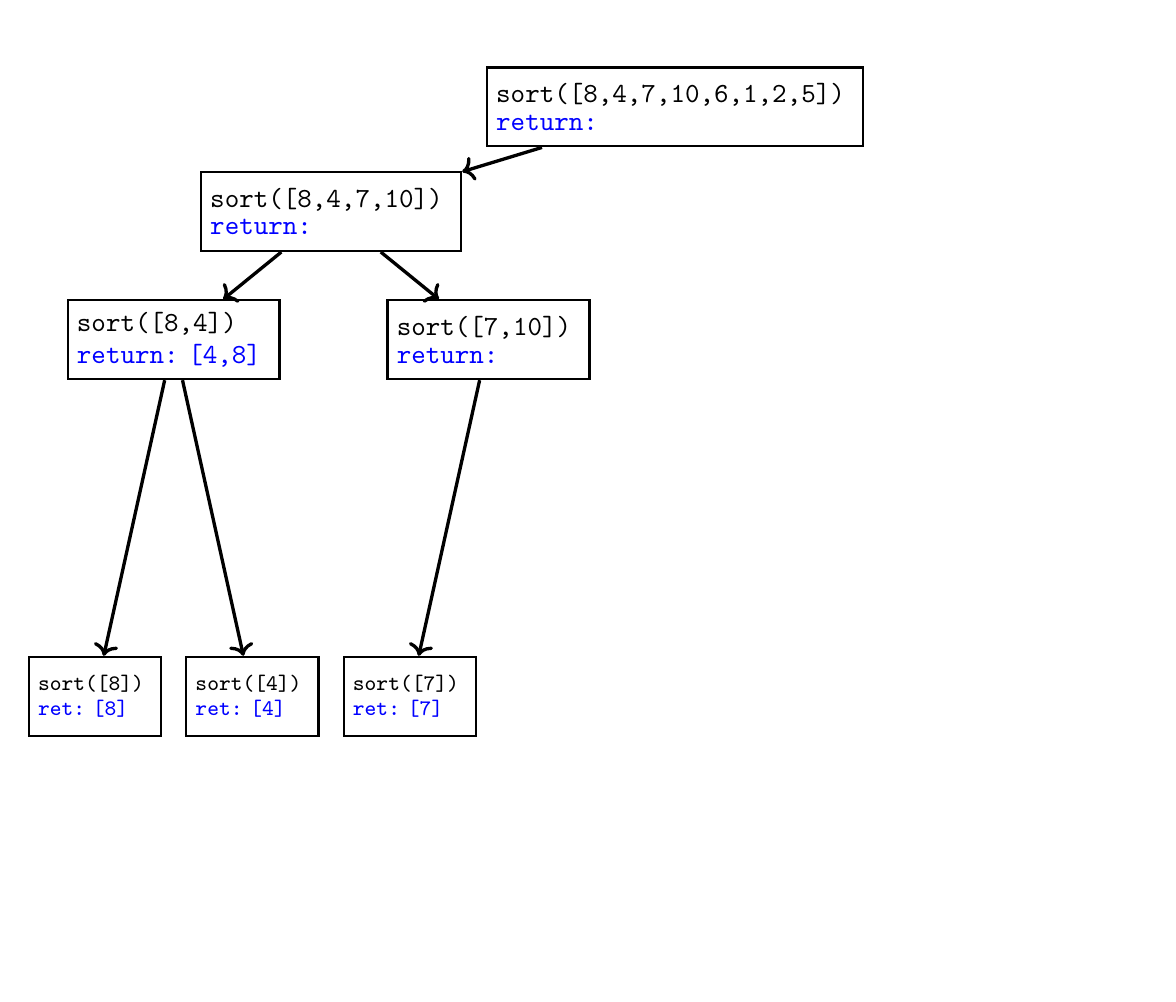
\begin{tikzpicture}[
    node distance=1cm,
    box/.style={rectangle, draw=black, thick,
                minimum width=1cm, minimum height=1cm, align=center}
]

\draw[draw = white] (-7,-6) rectangle (7,6);  % invisible bounding box

% Top node
\node[box] (root) at (1,5) {
  \texttt{\shortstack[l]{sort([8,4,7,10,6,1,2,5]) \\ \textcolor{blue}{return:}}}
};

% Level 1
\node[box, below left=\edgelen and \edgelen of root] (left)  {
 \texttt{\shortstack[l]{sort([8,4,7,10]) \\ \textcolor{blue}{return:}}}
};

\draw[->, very thick] (root) -- (left);

% Level 2 (left side)
\node[box, below=0.6cm of left, xshift=-2cm] (leftA) {
 \texttt{\shortstack[l]{sort([8,4]) \\ \textcolor{blue}{return:\!\!\!\! [4,8]}}}
};
\node[box, below=0.6cm of left, xshift=2cm] (leftB) {
 \texttt{\shortstack[l]{sort([7,10]) \\ \textcolor{blue}{return:}}}
};

\draw[->, very thick] (left) -- (leftA);
\draw[->, very thick] (left) -- (leftB);

% Level 3
\node[box, below=3.5cm of leftA, xshift=-1cm] (leftA1) { \footnotesize
 \texttt{\shortstack[l]{sort([8]) \\ \textcolor{blue}{ret:\!\!\!\! [8]}}}
};
\node[box, below=3.5cm of leftA, xshift=1cm] (leftA2) {\footnotesize
 \texttt{\shortstack[l]{sort([4]) \\ \textcolor{blue}{ret:\!\!\!\! [4]}}}
};

\node[box, below=3.5cm of leftB, xshift=-1cm] (leftB1) {\footnotesize
 \texttt{\shortstack[l]{sort([7]) \\ \textcolor{blue}{ret:\!\!\!\! [7]}}}
};



\draw[->, very thick] (leftA) -- (leftA1);
\draw[->, very thick] (leftA) -- (leftA2);
\draw[->, very thick] (leftB) -- (leftB1);


\end{tikzpicture}
}

\end{frame}





















\begin{frame}[fragile]{Étape 8}

\resizebox{0.90\textwidth}{!}{%
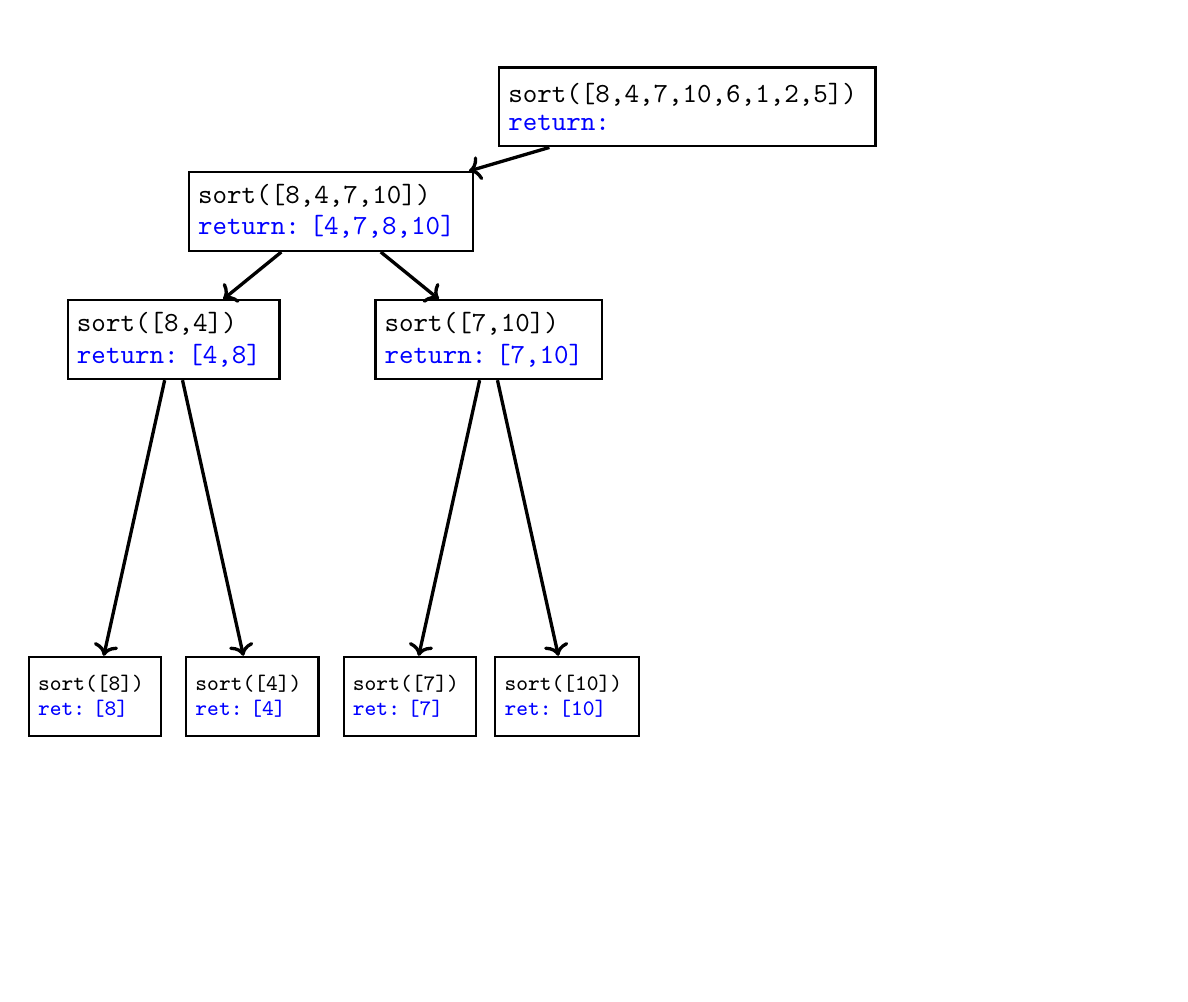
\begin{tikzpicture}[
    node distance=1cm,
    box/.style={rectangle, draw=black, thick,
                minimum width=1cm, minimum height=1cm, align=center}
]

\draw[draw = white] (-7,-6) rectangle (7,6);  % invisible bounding box

% Top node
\node[box] (root) at (1,5) {
  \texttt{\shortstack[l]{sort([8,4,7,10,6,1,2,5]) \\ \textcolor{blue}{return:}}}
};

% Level 1
\node[box, below left=\edgelen and \edgelen of root] (left)  {
 \texttt{\shortstack[l]{sort([8,4,7,10]) \\ \textcolor{blue}{return:\!\!\!\! [4,7,8,10]}}}
};

\draw[->, very thick] (root) -- (left);

% Level 2 (left side)
\node[box, below=0.6cm of left, xshift=-2cm] (leftA) {
 \texttt{\shortstack[l]{sort([8,4]) \\ \textcolor{blue}{return:\!\!\!\! [4,8]}}}
};
\node[box, below=0.6cm of left, xshift=2cm] (leftB) {
 \texttt{\shortstack[l]{sort([7,10]) \\ \textcolor{blue}{return:\!\!\!\! [7,10]}}}
};

\draw[->, very thick] (left) -- (leftA);
\draw[->, very thick] (left) -- (leftB);

% Level 3
\node[box, below=3.5cm of leftA, xshift=-1cm] (leftA1) { \footnotesize
 \texttt{\shortstack[l]{sort([8]) \\ \textcolor{blue}{ret:\!\!\!\! [8]}}}
};
\node[box, below=3.5cm of leftA, xshift=1cm] (leftA2) {\footnotesize
 \texttt{\shortstack[l]{sort([4]) \\ \textcolor{blue}{ret:\!\!\!\! [4]}}}
};

\node[box, below=3.5cm of leftB, xshift=-1cm] (leftB1) {\footnotesize
 \texttt{\shortstack[l]{sort([7]) \\ \textcolor{blue}{ret:\!\!\!\! [7]}}}
};

\node[box, below=3.5cm of leftB, xshift=1cm] (leftB2) {\footnotesize
 \texttt{\shortstack[l]{sort([10]) \\ \textcolor{blue}{ret:\!\!\!\! [10]}}}
};

\draw[->, very thick] (leftA) -- (leftA1);
\draw[->, very thick] (leftA) -- (leftA2);
\draw[->, very thick] (leftB) -- (leftB1);
\draw[->, very thick] (leftB) -- (leftB2);


\end{tikzpicture}
}

\end{frame}
























\begin{frame}[fragile]{Étape 9}

\resizebox{0.92\textwidth}{!}{%
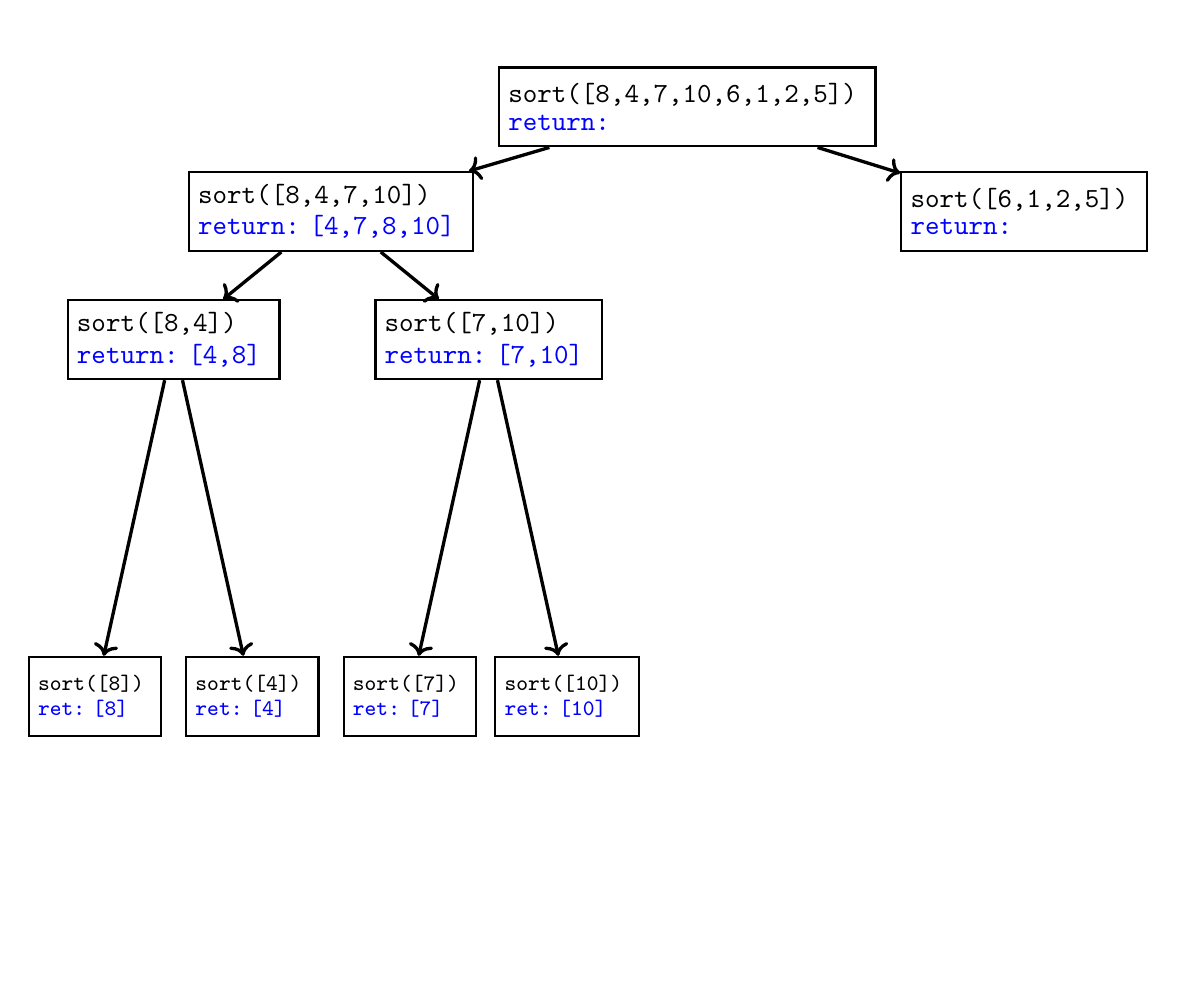
\begin{tikzpicture}[
    node distance=1cm,
    box/.style={rectangle, draw=black, thick,
                minimum width=1cm, minimum height=1cm, align=center}
]

\draw[draw = white] (-7,-6) rectangle (7,6);  % invisible bounding box

% Top node
\node[box] (root) at (1,5) {
  \texttt{\shortstack[l]{sort([8,4,7,10,6,1,2,5]) \\ \textcolor{blue}{return:}}}
};

% Level 1
\node[box, below left=\edgelen and \edgelen of root] (left)  {
 \texttt{\shortstack[l]{sort([8,4,7,10]) \\ \textcolor{blue}{return:\!\!\!\! [4,7,8,10]}}}
};
\node[box, below right=\edgelen and \edgelen of root] (right)  {
 \texttt{\shortstack[l]{sort([6,1,2,5]) \\ \textcolor{blue}{return:}}}
};
\draw[->, very thick] (root) -- (left);
\draw[->, very thick] (root) -- (right);

% Level 2 (left side)
\node[box, below=0.6cm of left, xshift=-2cm] (leftA) {
 \texttt{\shortstack[l]{sort([8,4]) \\ \textcolor{blue}{return:\!\!\!\! [4,8]}}}
};
\node[box, below=0.6cm of left, xshift=2cm] (leftB) {
 \texttt{\shortstack[l]{sort([7,10]) \\ \textcolor{blue}{return:\!\!\!\! [7,10]}}}
};

\draw[->, very thick] (left) -- (leftA);
\draw[->, very thick] (left) -- (leftB);

% Level 3
\node[box, below=3.5cm of leftA, xshift=-1cm] (leftA1) { \footnotesize
 \texttt{\shortstack[l]{sort([8]) \\ \textcolor{blue}{ret:\!\!\!\! [8]}}}
};
\node[box, below=3.5cm of leftA, xshift=1cm] (leftA2) {\footnotesize
 \texttt{\shortstack[l]{sort([4]) \\ \textcolor{blue}{ret:\!\!\!\! [4]}}}
};

\node[box, below=3.5cm of leftB, xshift=-1cm] (leftB1) {\footnotesize
 \texttt{\shortstack[l]{sort([7]) \\ \textcolor{blue}{ret:\!\!\!\! [7]}}}
};

\node[box, below=3.5cm of leftB, xshift=1cm] (leftB2) {\footnotesize
 \texttt{\shortstack[l]{sort([10]) \\ \textcolor{blue}{ret:\!\!\!\! [10]}}}
};

\draw[->, very thick] (leftA) -- (leftA1);
\draw[->, very thick] (leftA) -- (leftA2);
\draw[->, very thick] (leftB) -- (leftB1);
\draw[->, very thick] (leftB) -- (leftB2);


\end{tikzpicture}
}

\end{frame}














\begin{frame}[fragile]{Étape 10}

\resizebox{0.92\textwidth}{!}{%
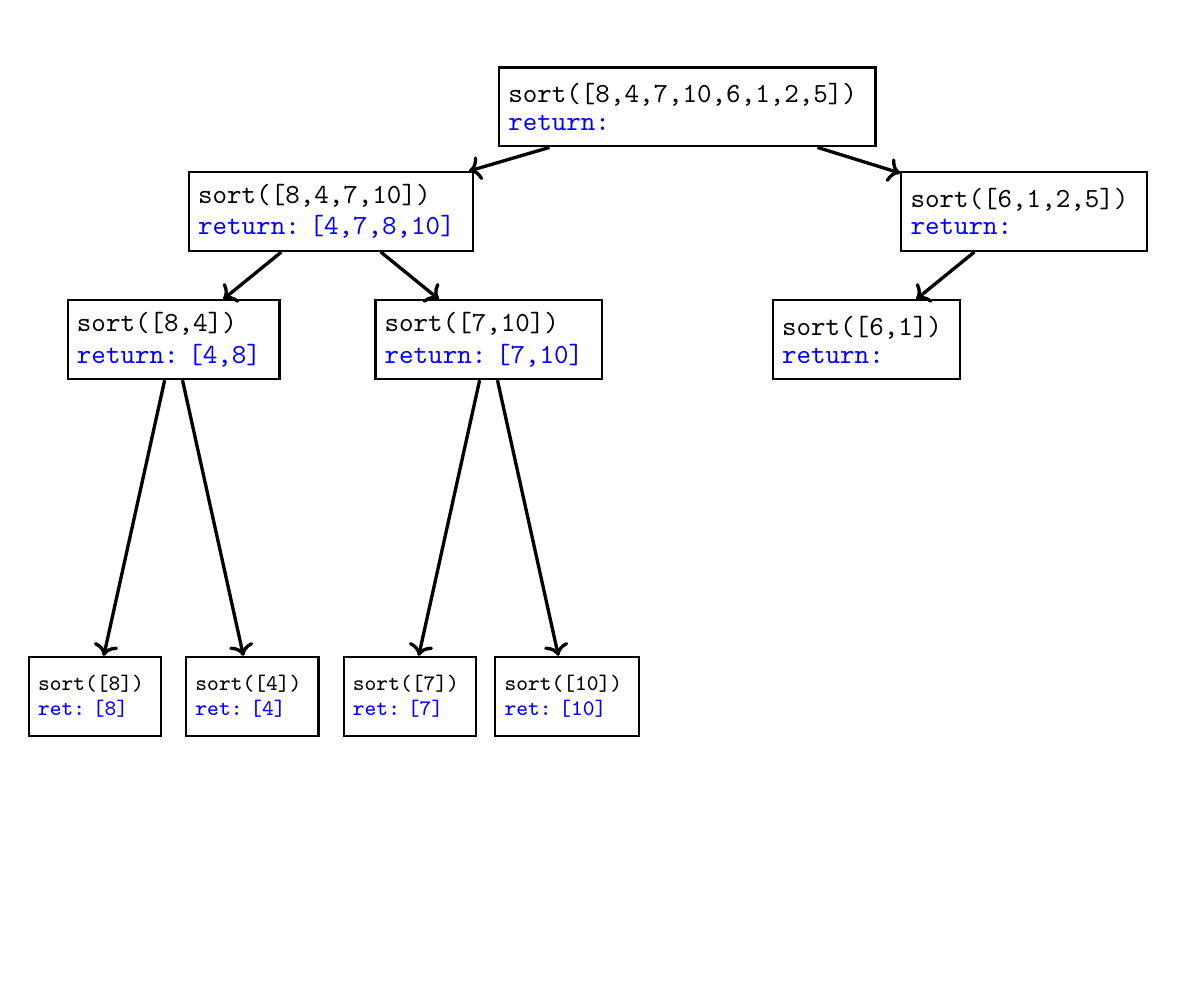
\begin{tikzpicture}[
    node distance=1cm,
    box/.style={rectangle, draw=black, thick,
                minimum width=1cm, minimum height=1cm, align=center}
]

\draw[draw = white] (-7,-6) rectangle (7,6);  % invisible bounding box

% Top node
\node[box] (root) at (1,5) {
  \texttt{\shortstack[l]{sort([8,4,7,10,6,1,2,5]) \\ \textcolor{blue}{return:}}}
};

% Level 1
\node[box, below left=\edgelen and \edgelen of root] (left)  {
 \texttt{\shortstack[l]{sort([8,4,7,10]) \\ \textcolor{blue}{return:\!\!\!\! [4,7,8,10]}}}
};
\node[box, below right=\edgelen and \edgelen of root] (right)  {
 \texttt{\shortstack[l]{sort([6,1,2,5]) \\ \textcolor{blue}{return:}}}
};
\draw[->, very thick] (root) -- (left);
\draw[->, very thick] (root) -- (right);

% Level 2 (left side)
\node[box, below=0.6cm of left, xshift=-2cm] (leftA) {
 \texttt{\shortstack[l]{sort([8,4]) \\ \textcolor{blue}{return:\!\!\!\! [4,8]}}}
};
\node[box, below=0.6cm of left, xshift=2cm] (leftB) {
 \texttt{\shortstack[l]{sort([7,10]) \\ \textcolor{blue}{return:\!\!\!\! [7,10]}}}
};

\node[box, below=0.6cm of right, xshift=-2cm] (rightA) {
 \texttt{\shortstack[l]{sort([6,1]) \\ \textcolor{blue}{return:}}}
};

\draw[->, very thick] (left) -- (leftA);
\draw[->, very thick] (left) -- (leftB);
\draw[->, very thick] (right) -- (rightA);

% Level 3
\node[box, below=3.5cm of leftA, xshift=-1cm] (leftA1) { \footnotesize
 \texttt{\shortstack[l]{sort([8]) \\ \textcolor{blue}{ret:\!\!\!\! [8]}}}
};
\node[box, below=3.5cm of leftA, xshift=1cm] (leftA2) {\footnotesize
 \texttt{\shortstack[l]{sort([4]) \\ \textcolor{blue}{ret:\!\!\!\! [4]}}}
};

\node[box, below=3.5cm of leftB, xshift=-1cm] (leftB1) {\footnotesize
 \texttt{\shortstack[l]{sort([7]) \\ \textcolor{blue}{ret:\!\!\!\! [7]}}}
};

\node[box, below=3.5cm of leftB, xshift=1cm] (leftB2) {\footnotesize
 \texttt{\shortstack[l]{sort([10]) \\ \textcolor{blue}{ret:\!\!\!\! [10]}}}
};

\draw[->, very thick] (leftA) -- (leftA1);
\draw[->, very thick] (leftA) -- (leftA2);
\draw[->, very thick] (leftB) -- (leftB1);
\draw[->, very thick] (leftB) -- (leftB2);


\end{tikzpicture}
}
\end{frame}








\begin{frame}[fragile]{Étape 11}

\resizebox{0.92\textwidth}{!}{%
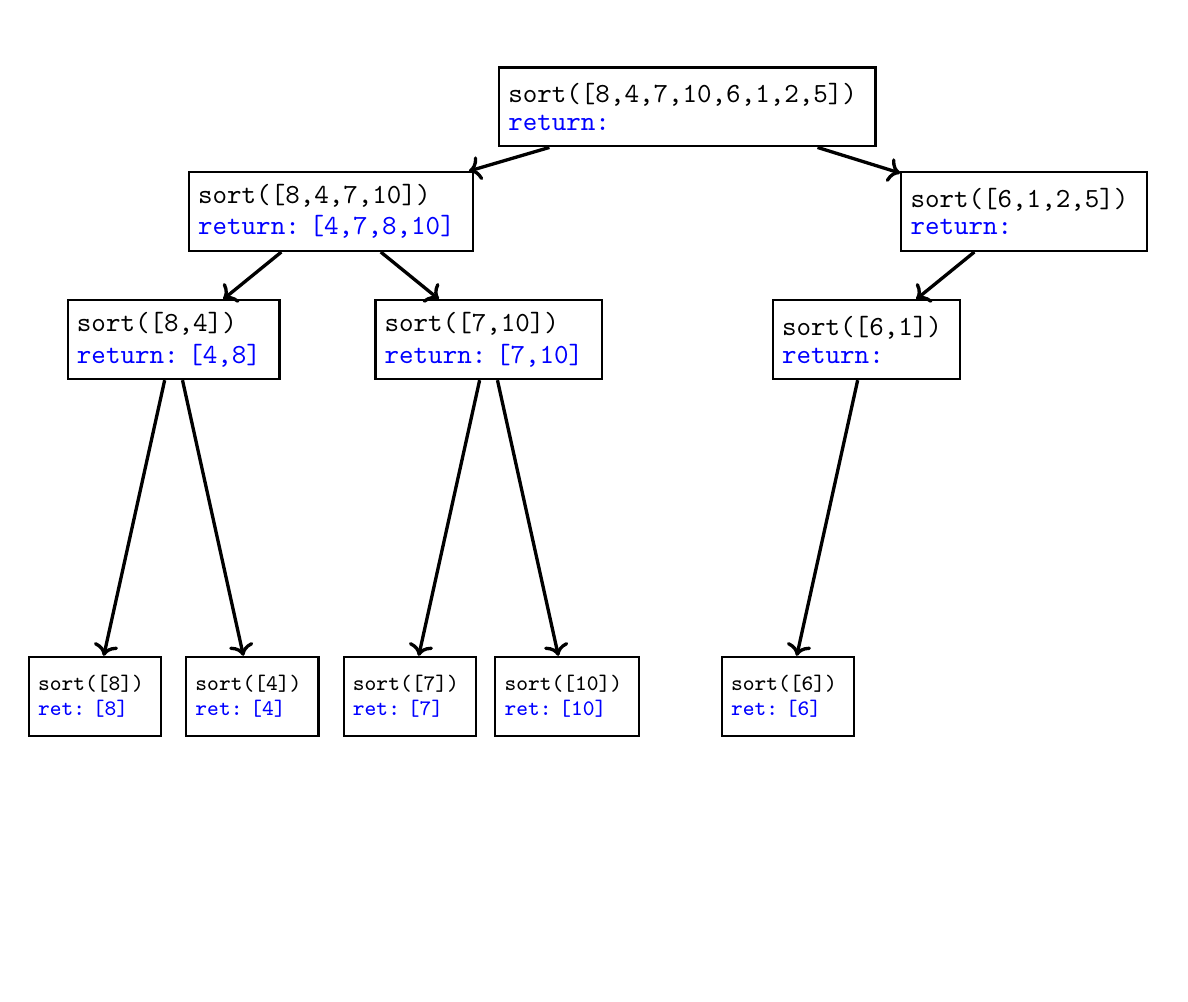
\begin{tikzpicture}[
    node distance=1cm,
    box/.style={rectangle, draw=black, thick,
                minimum width=1cm, minimum height=1cm, align=center}
]

\draw[draw = white] (-7,-6) rectangle (7,6);  % invisible bounding box

% Top node
\node[box] (root) at (1,5) {
  \texttt{\shortstack[l]{sort([8,4,7,10,6,1,2,5]) \\ \textcolor{blue}{return:}}}
};

% Level 1
\node[box, below left=\edgelen and \edgelen of root] (left)  {
 \texttt{\shortstack[l]{sort([8,4,7,10]) \\ \textcolor{blue}{return:\!\!\!\! [4,7,8,10]}}}
};
\node[box, below right=\edgelen and \edgelen of root] (right)  {
 \texttt{\shortstack[l]{sort([6,1,2,5]) \\ \textcolor{blue}{return:}}}
};
\draw[->, very thick] (root) -- (left);
\draw[->, very thick] (root) -- (right);

% Level 2 (left side)
\node[box, below=0.6cm of left, xshift=-2cm] (leftA) {
 \texttt{\shortstack[l]{sort([8,4]) \\ \textcolor{blue}{return:\!\!\!\! [4,8]}}}
};
\node[box, below=0.6cm of left, xshift=2cm] (leftB) {
 \texttt{\shortstack[l]{sort([7,10]) \\ \textcolor{blue}{return:\!\!\!\! [7,10]}}}
};

\node[box, below=0.6cm of right, xshift=-2cm] (rightA) {
 \texttt{\shortstack[l]{sort([6,1]) \\ \textcolor{blue}{return:}}}
};

\draw[->, very thick] (left) -- (leftA);
\draw[->, very thick] (left) -- (leftB);
\draw[->, very thick] (right) -- (rightA);

% Level 3
\node[box, below=3.5cm of leftA, xshift=-1cm] (leftA1) { \footnotesize
 \texttt{\shortstack[l]{sort([8]) \\ \textcolor{blue}{ret:\!\!\!\! [8]}}}
};
\node[box, below=3.5cm of leftA, xshift=1cm] (leftA2) {\footnotesize
 \texttt{\shortstack[l]{sort([4]) \\ \textcolor{blue}{ret:\!\!\!\! [4]}}}
};

\node[box, below=3.5cm of leftB, xshift=-1cm] (leftB1) {\footnotesize
 \texttt{\shortstack[l]{sort([7]) \\ \textcolor{blue}{ret:\!\!\!\! [7]}}}
};

\node[box, below=3.5cm of leftB, xshift=1cm] (leftB2) {\footnotesize
 \texttt{\shortstack[l]{sort([10]) \\ \textcolor{blue}{ret:\!\!\!\! [10]}}}
};

\node[box, below=3.5cm of rightA, xshift=-1cm] (rightA1) {\footnotesize
 \texttt{\shortstack[l]{sort([6]) \\ \textcolor{blue}{ret:\!\!\!\! [6]}}}
};

% \node[box, below=3.5cm of rightA, xshift=1cm] (rightA2) {\footnotesize
%  \texttt{\shortstack[l]{sort([1]) \\ \textcolor{blue}{ret:\!\!\!\! [1]}}}
% };

\draw[->, very thick] (leftA) -- (leftA1);
\draw[->, very thick] (leftA) -- (leftA2);
\draw[->, very thick] (leftB) -- (leftB1);
\draw[->, very thick] (leftB) -- (leftB2);
\draw[->, very thick] (rightA) -- (rightA1);



\end{tikzpicture}
}
\end{frame}















\begin{frame}[fragile]{Étape 12}
\resizebox{0.92\textwidth}{!}{%
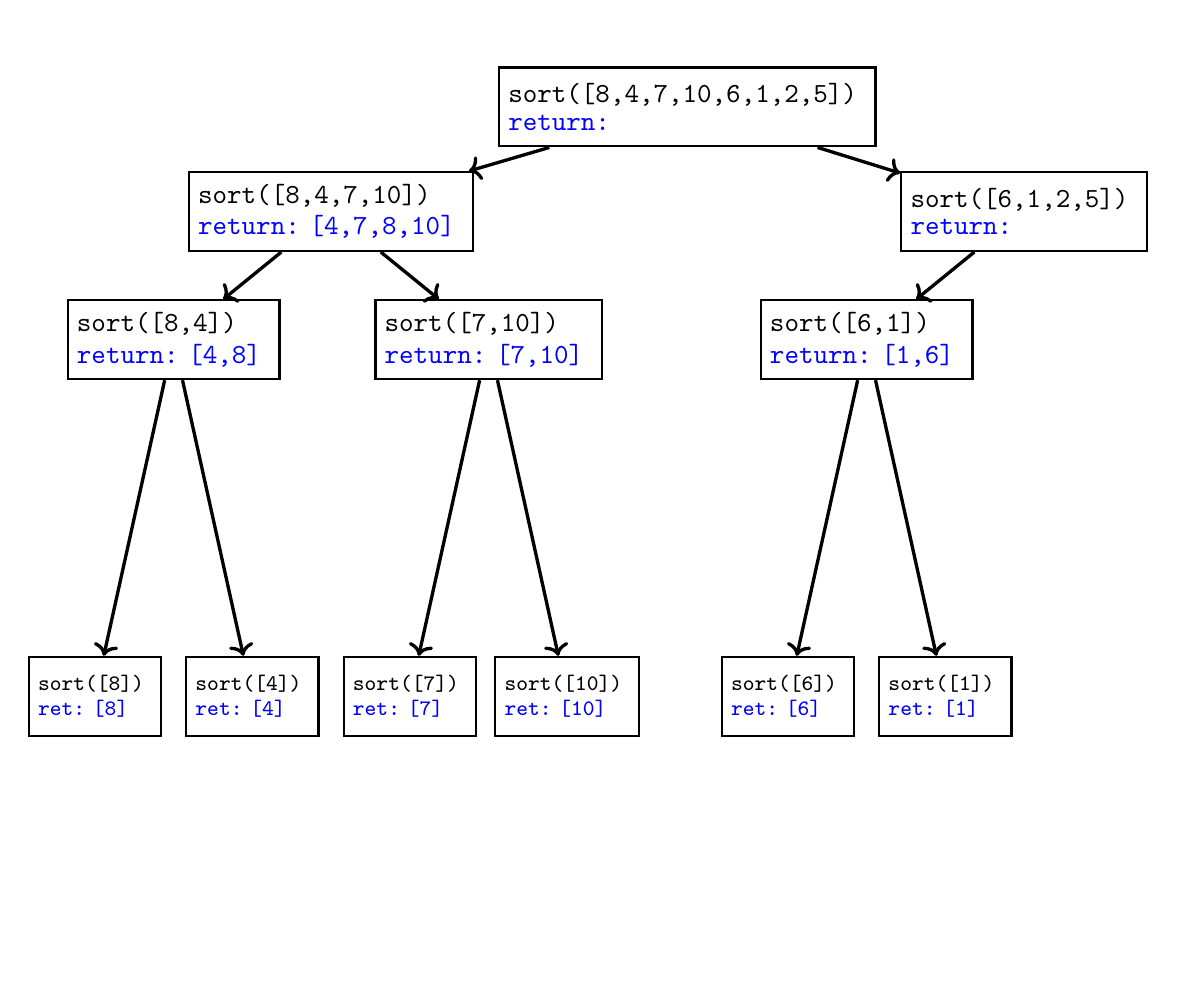
\begin{tikzpicture}[
    node distance=1cm,
    box/.style={rectangle, draw=black, thick,
                minimum width=1cm, minimum height=1cm, align=center}
]

\draw[draw = white] (-7,-6) rectangle (7,6);  % invisible bounding box

% Top node
\node[box] (root) at (1,5) {
  \texttt{\shortstack[l]{sort([8,4,7,10,6,1,2,5]) \\ \textcolor{blue}{return:}}}
};

% Level 1
\node[box, below left=\edgelen and \edgelen of root] (left)  {
 \texttt{\shortstack[l]{sort([8,4,7,10]) \\ \textcolor{blue}{return:\!\!\!\! [4,7,8,10]}}}
};
\node[box, below right=\edgelen and \edgelen of root] (right)  {
 \texttt{\shortstack[l]{sort([6,1,2,5]) \\ \textcolor{blue}{return:}}}
};
\draw[->, very thick] (root) -- (left);
\draw[->, very thick] (root) -- (right);

% Level 2 (left side)
\node[box, below=0.6cm of left, xshift=-2cm] (leftA) {
 \texttt{\shortstack[l]{sort([8,4]) \\ \textcolor{blue}{return:\!\!\!\! [4,8]}}}
};
\node[box, below=0.6cm of left, xshift=2cm] (leftB) {
 \texttt{\shortstack[l]{sort([7,10]) \\ \textcolor{blue}{return:\!\!\!\! [7,10]}}}
};

\node[box, below=0.6cm of right, xshift=-2cm] (rightA) {
 \texttt{\shortstack[l]{sort([6,1]) \\ \textcolor{blue}{return:\!\!\!\! [1,6]}}}
};


\draw[->, very thick] (left) -- (leftA);
\draw[->, very thick] (left) -- (leftB);
\draw[->, very thick] (right) -- (rightA);


% Level 3
\node[box, below=3.5cm of leftA, xshift=-1cm] (leftA1) { \footnotesize
 \texttt{\shortstack[l]{sort([8]) \\ \textcolor{blue}{ret:\!\!\!\! [8]}}}
};
\node[box, below=3.5cm of leftA, xshift=1cm] (leftA2) {\footnotesize
 \texttt{\shortstack[l]{sort([4]) \\ \textcolor{blue}{ret:\!\!\!\! [4]}}}
};

\node[box, below=3.5cm of leftB, xshift=-1cm] (leftB1) {\footnotesize
 \texttt{\shortstack[l]{sort([7]) \\ \textcolor{blue}{ret:\!\!\!\! [7]}}}
};

\node[box, below=3.5cm of leftB, xshift=1cm] (leftB2) {\footnotesize
 \texttt{\shortstack[l]{sort([10]) \\ \textcolor{blue}{ret:\!\!\!\! [10]}}}
};

\node[box, below=3.5cm of rightA, xshift=-1cm] (rightA1) {\footnotesize
 \texttt{\shortstack[l]{sort([6]) \\ \textcolor{blue}{ret:\!\!\!\! [6]}}}
};

\node[box, below=3.5cm of rightA, xshift=1cm] (rightA2) {\footnotesize
 \texttt{\shortstack[l]{sort([1]) \\ \textcolor{blue}{ret:\!\!\!\! [1]}}}
};

\draw[->, very thick] (leftA) -- (leftA1);
\draw[->, very thick] (leftA) -- (leftA2);
\draw[->, very thick] (leftB) -- (leftB1);
\draw[->, very thick] (leftB) -- (leftB2);
\draw[->, very thick] (rightA) -- (rightA1);
\draw[->, very thick] (rightA) -- (rightA2);


\end{tikzpicture}
}

\end{frame}




















\begin{frame}[fragile]{Étape 13}
\resizebox{1.02\textwidth}{!}{%
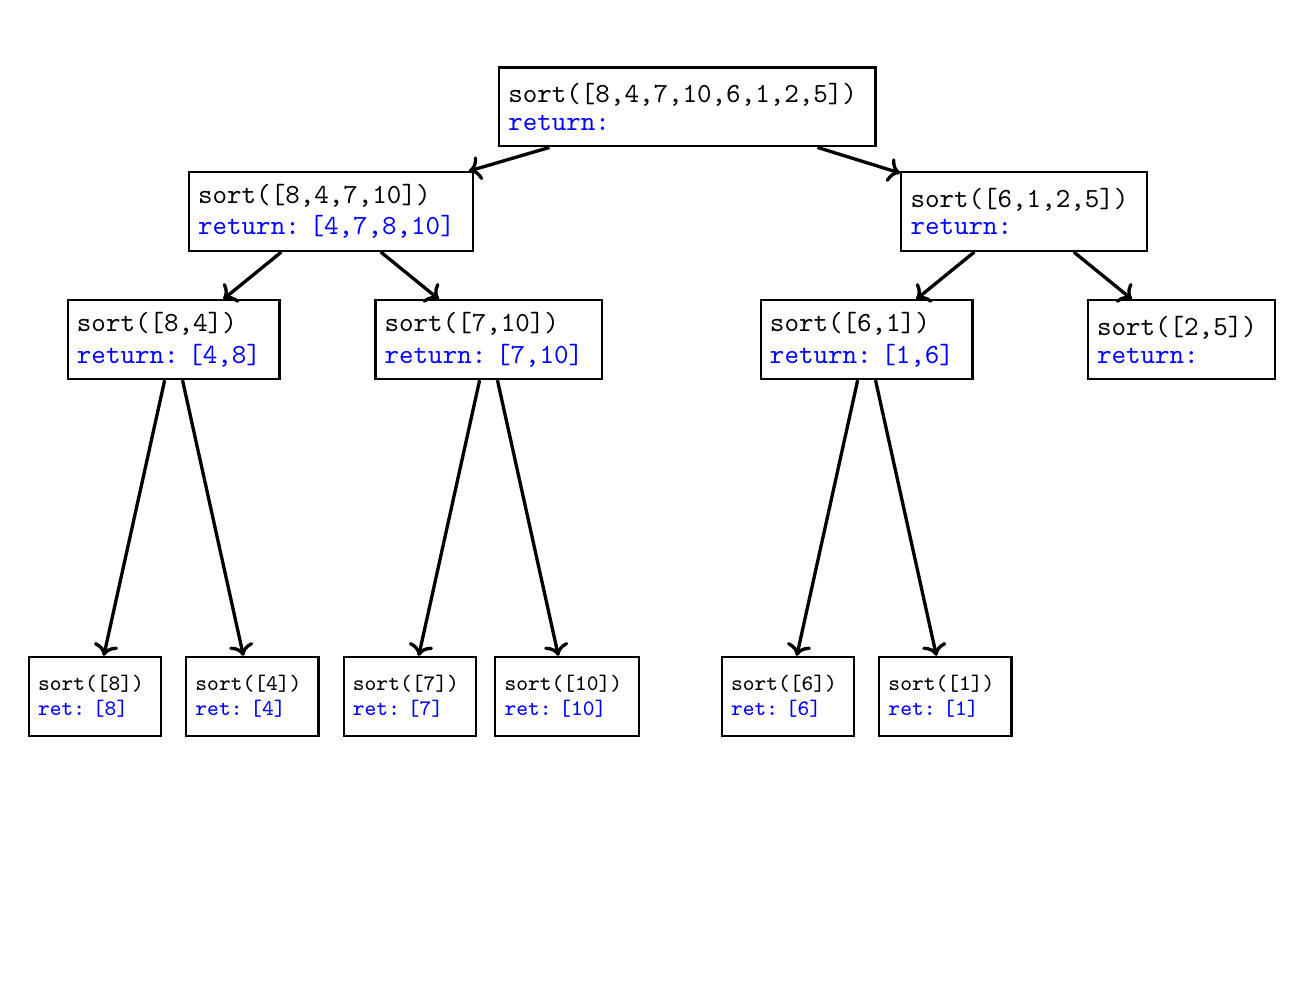
\begin{tikzpicture}[
    node distance=1cm,
    box/.style={rectangle, draw=black, thick,
                minimum width=1cm, minimum height=1cm, align=center}
]

\draw[draw = white] (-7,-6) rectangle (7,6);  % invisible bounding box

% Top node
\node[box] (root) at (1,5) {
  \texttt{\shortstack[l]{sort([8,4,7,10,6,1,2,5]) \\ \textcolor{blue}{return:}}}
};

% Level 1
\node[box, below left=\edgelen and \edgelen of root] (left)  {
 \texttt{\shortstack[l]{sort([8,4,7,10]) \\ \textcolor{blue}{return:\!\!\!\! [4,7,8,10]}}}
};
\node[box, below right=\edgelen and \edgelen of root] (right)  {
 \texttt{\shortstack[l]{sort([6,1,2,5]) \\ \textcolor{blue}{return:}}}
};
\draw[->, very thick] (root) -- (left);
\draw[->, very thick] (root) -- (right);

% Level 2 (left side)
\node[box, below=0.6cm of left, xshift=-2cm] (leftA) {
 \texttt{\shortstack[l]{sort([8,4]) \\ \textcolor{blue}{return:\!\!\!\! [4,8]}}}
};
\node[box, below=0.6cm of left, xshift=2cm] (leftB) {
 \texttt{\shortstack[l]{sort([7,10]) \\ \textcolor{blue}{return:\!\!\!\! [7,10]}}}
};

\node[box, below=0.6cm of right, xshift=-2cm] (rightA) {
 \texttt{\shortstack[l]{sort([6,1]) \\ \textcolor{blue}{return:\!\!\!\! [1,6]}}}
};

\node[box, below=0.6cm of right, xshift=2cm] (rightB) {
 \texttt{\shortstack[l]{sort([2,5]) \\ \textcolor{blue}{return:}}}
};

\draw[->, very thick] (left) -- (leftA);
\draw[->, very thick] (left) -- (leftB);
\draw[->, very thick] (right) -- (rightA);
\draw[->, very thick] (right) -- (rightB);


% Level 3
\node[box, below=3.5cm of leftA, xshift=-1cm] (leftA1) { \footnotesize
 \texttt{\shortstack[l]{sort([8]) \\ \textcolor{blue}{ret:\!\!\!\! [8]}}}
};
\node[box, below=3.5cm of leftA, xshift=1cm] (leftA2) {\footnotesize
 \texttt{\shortstack[l]{sort([4]) \\ \textcolor{blue}{ret:\!\!\!\! [4]}}}
};

\node[box, below=3.5cm of leftB, xshift=-1cm] (leftB1) {\footnotesize
 \texttt{\shortstack[l]{sort([7]) \\ \textcolor{blue}{ret:\!\!\!\! [7]}}}
};

\node[box, below=3.5cm of leftB, xshift=1cm] (leftB2) {\footnotesize
 \texttt{\shortstack[l]{sort([10]) \\ \textcolor{blue}{ret:\!\!\!\! [10]}}}
};

\node[box, below=3.5cm of rightA, xshift=-1cm] (rightA1) {\footnotesize
 \texttt{\shortstack[l]{sort([6]) \\ \textcolor{blue}{ret:\!\!\!\! [6]}}}
};

\node[box, below=3.5cm of rightA, xshift=1cm] (rightA2) {\footnotesize
 \texttt{\shortstack[l]{sort([1]) \\ \textcolor{blue}{ret:\!\!\!\! [1]}}}
};

\draw[->, very thick] (leftA) -- (leftA1);
\draw[->, very thick] (leftA) -- (leftA2);
\draw[->, very thick] (leftB) -- (leftB1);
\draw[->, very thick] (leftB) -- (leftB2);
\draw[->, very thick] (rightA) -- (rightA1);
\draw[->, very thick] (rightA) -- (rightA2);


\end{tikzpicture}
}


\end{frame}





















\begin{frame}[fragile]{Étape 14}

\resizebox{1.051\textwidth}{!}{%
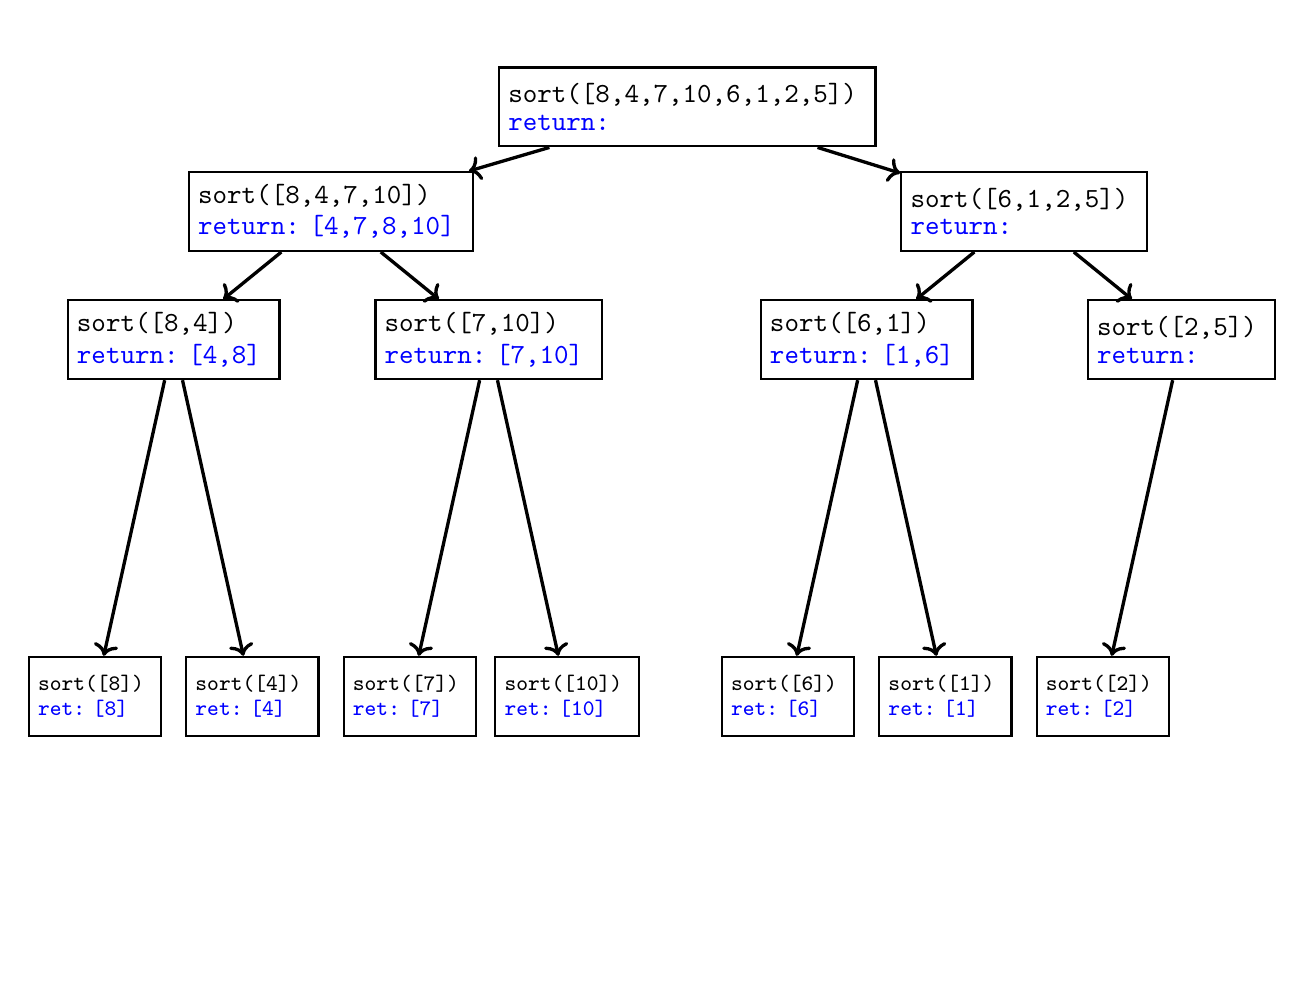
\begin{tikzpicture}[
    node distance=1cm,
    box/.style={rectangle, draw=black, thick,
                minimum width=1cm, minimum height=1cm, align=center}
]

\draw[draw = white] (-7,-6) rectangle (7,6);  % invisible bounding box

% Top node
\node[box] (root) at (1,5) {
  \texttt{\shortstack[l]{sort([8,4,7,10,6,1,2,5]) \\ \textcolor{blue}{return:}}}
};

% Level 1
\node[box, below left=\edgelen and \edgelen of root] (left)  {
 \texttt{\shortstack[l]{sort([8,4,7,10]) \\ \textcolor{blue}{return:\!\!\!\! [4,7,8,10]}}}
};
\node[box, below right=\edgelen and \edgelen of root] (right)  {
 \texttt{\shortstack[l]{sort([6,1,2,5]) \\ \textcolor{blue}{return:}}}
};
\draw[->, very thick] (root) -- (left);
\draw[->, very thick] (root) -- (right);

% Level 2 (left side)
\node[box, below=0.6cm of left, xshift=-2cm] (leftA) {
 \texttt{\shortstack[l]{sort([8,4]) \\ \textcolor{blue}{return:\!\!\!\! [4,8]}}}
};
\node[box, below=0.6cm of left, xshift=2cm] (leftB) {
 \texttt{\shortstack[l]{sort([7,10]) \\ \textcolor{blue}{return:\!\!\!\! [7,10]}}}
};

\node[box, below=0.6cm of right, xshift=-2cm] (rightA) {
 \texttt{\shortstack[l]{sort([6,1]) \\ \textcolor{blue}{return:\!\!\!\! [1,6]}}}
};

\node[box, below=0.6cm of right, xshift=2cm] (rightB) {
 \texttt{\shortstack[l]{sort([2,5]) \\ \textcolor{blue}{return:}}}
};

\draw[->, very thick] (left) -- (leftA);
\draw[->, very thick] (left) -- (leftB);
\draw[->, very thick] (right) -- (rightA);
\draw[->, very thick] (right) -- (rightB);


% Level 3
\node[box, below=3.5cm of leftA, xshift=-1cm] (leftA1) { \footnotesize
 \texttt{\shortstack[l]{sort([8]) \\ \textcolor{blue}{ret:\!\!\!\! [8]}}}
};
\node[box, below=3.5cm of leftA, xshift=1cm] (leftA2) {\footnotesize
 \texttt{\shortstack[l]{sort([4]) \\ \textcolor{blue}{ret:\!\!\!\! [4]}}}
};

\node[box, below=3.5cm of leftB, xshift=-1cm] (leftB1) {\footnotesize
 \texttt{\shortstack[l]{sort([7]) \\ \textcolor{blue}{ret:\!\!\!\! [7]}}}
};

\node[box, below=3.5cm of leftB, xshift=1cm] (leftB2) {\footnotesize
 \texttt{\shortstack[l]{sort([10]) \\ \textcolor{blue}{ret:\!\!\!\! [10]}}}
};

\node[box, below=3.5cm of rightA, xshift=-1cm] (rightA1) {\footnotesize
 \texttt{\shortstack[l]{sort([6]) \\ \textcolor{blue}{ret:\!\!\!\! [6]}}}
};

\node[box, below=3.5cm of rightA, xshift=1cm] (rightA2) {\footnotesize
 \texttt{\shortstack[l]{sort([1]) \\ \textcolor{blue}{ret:\!\!\!\! [1]}}}
};


\node[box, below=3.5cm of rightB, xshift=-1cm] (rightB1) {\footnotesize
 \texttt{\shortstack[l]{sort([2]) \\ \textcolor{blue}{ret:\!\!\!\! [2]}}}
};


\draw[->, very thick] (leftA) -- (leftA1);
\draw[->, very thick] (leftA) -- (leftA2);
\draw[->, very thick] (leftB) -- (leftB1);
\draw[->, very thick] (leftB) -- (leftB2);
\draw[->, very thick] (rightA) -- (rightA1);
\draw[->, very thick] (rightA) -- (rightA2);
\draw[->, very thick] (rightB) -- (rightB1);


\end{tikzpicture}
}


\end{frame}





\begin{frame}[fragile]{Étape 15}
\hspace*{-0.3cm}
\resizebox{1.08\textwidth}{!}{%
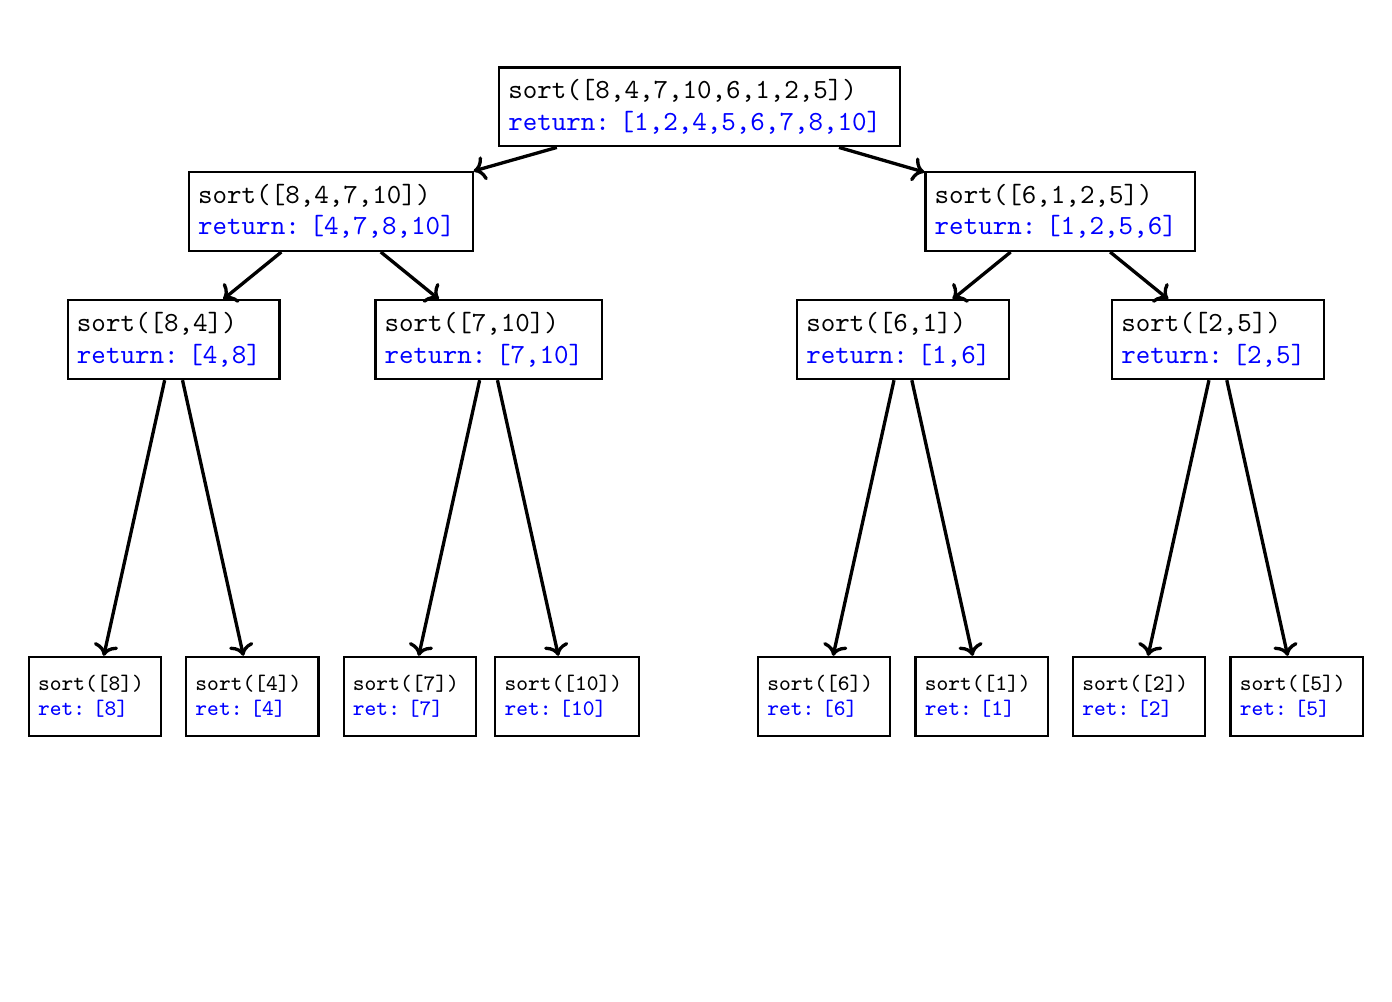
\begin{tikzpicture}[
    node distance=1cm,
    box/.style={rectangle, draw=black, thick,
                minimum width=1cm, minimum height=1cm, align=center}
]

\draw[draw = white] (-7,-6) rectangle (7,6);  % invisible bounding box

% Top node
\node[box] (root) at (1,5) {
  \texttt{\shortstack[l]{sort([8,4,7,10,6,1,2,5]) \\ \textcolor{blue}{return:\!\!\!\! [1,2,4,5,6,7,8,10]}}}
};

% Level 1
\node[box, below left=\edgelen and \edgelen of root] (left)  {
 \texttt{\shortstack[l]{sort([8,4,7,10]) \\ \textcolor{blue}{return:\!\!\!\! [4,7,8,10]}}}
};
\node[box, below right=\edgelen and \edgelen of root] (right)  {
 \texttt{\shortstack[l]{sort([6,1,2,5]) \\ \textcolor{blue}{return:\!\!\!\! [1,2,5,6]}}}
};
\draw[->, very thick] (root) -- (left);
\draw[->, very thick] (root) -- (right);

% Level 2 (left side)
\node[box, below=0.6cm of left, xshift=-2cm] (leftA) {
 \texttt{\shortstack[l]{sort([8,4]) \\ \textcolor{blue}{return:\!\!\!\! [4,8]}}}
};
\node[box, below=0.6cm of left, xshift=2cm] (leftB) {
 \texttt{\shortstack[l]{sort([7,10]) \\ \textcolor{blue}{return:\!\!\!\! [7,10]}}}
};

\node[box, below=0.6cm of right, xshift=-2cm] (rightA) {
 \texttt{\shortstack[l]{sort([6,1]) \\ \textcolor{blue}{return:\!\!\!\! [1,6]}}}
};

\node[box, below=0.6cm of right, xshift=2cm] (rightB) {
 \texttt{\shortstack[l]{sort([2,5]) \\ \textcolor{blue}{return:\!\!\!\! [2,5]}}}
};

\draw[->, very thick] (left) -- (leftA);
\draw[->, very thick] (left) -- (leftB);
\draw[->, very thick] (right) -- (rightA);
\draw[->, very thick] (right) -- (rightB);


% Level 3
\node[box, below=3.5cm of leftA, xshift=-1cm] (leftA1) { \footnotesize
 \texttt{\shortstack[l]{sort([8]) \\ \textcolor{blue}{ret:\!\!\!\! [8]}}}
};
\node[box, below=3.5cm of leftA, xshift=1cm] (leftA2) {\footnotesize
 \texttt{\shortstack[l]{sort([4]) \\ \textcolor{blue}{ret:\!\!\!\! [4]}}}
};

\node[box, below=3.5cm of leftB, xshift=-1cm] (leftB1) {\footnotesize
 \texttt{\shortstack[l]{sort([7]) \\ \textcolor{blue}{ret:\!\!\!\! [7]}}}
};

\node[box, below=3.5cm of leftB, xshift=1cm] (leftB2) {\footnotesize
 \texttt{\shortstack[l]{sort([10]) \\ \textcolor{blue}{ret:\!\!\!\! [10]}}}
};

\node[box, below=3.5cm of rightA, xshift=-1cm] (rightA1) {\footnotesize
 \texttt{\shortstack[l]{sort([6]) \\ \textcolor{blue}{ret:\!\!\!\! [6]}}}
};

\node[box, below=3.5cm of rightA, xshift=1cm] (rightA2) {\footnotesize
 \texttt{\shortstack[l]{sort([1]) \\ \textcolor{blue}{ret:\!\!\!\! [1]}}}
};


\node[box, below=3.5cm of rightB, xshift=-1cm] (rightB1) {\footnotesize
 \texttt{\shortstack[l]{sort([2]) \\ \textcolor{blue}{ret:\!\!\!\! [2]}}}
};

\node[box, below=3.5cm of rightB, xshift=1cm] (rightB2) {\footnotesize
 \texttt{\shortstack[l]{sort([5]) \\ \textcolor{blue}{ret:\!\!\!\! [5]}}}
};

\draw[->, very thick] (leftA) -- (leftA1);
\draw[->, very thick] (leftA) -- (leftA2);
\draw[->, very thick] (leftB) -- (leftB1);
\draw[->, very thick] (leftB) -- (leftB2);
\draw[->, very thick] (rightA) -- (rightA1);
\draw[->, very thick] (rightA) -- (rightA2);
\draw[->, very thick] (rightB) -- (rightB1);
\draw[->, very thick] (rightB) -- (rightB2);


\end{tikzpicture}
}


\end{frame}

\end{document}